\section{Background and Motivation}
\label{sec:background}

\begin{figure}[t]
   \centering
   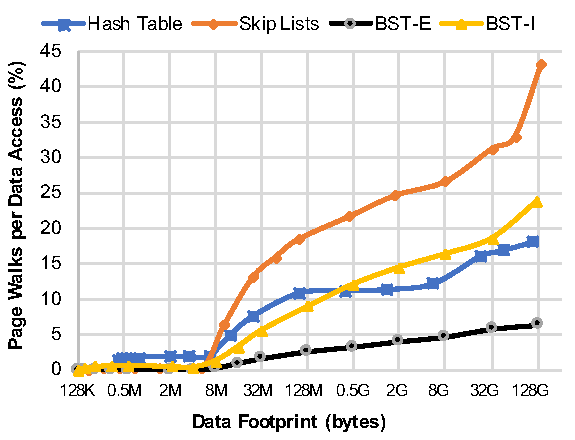
\includegraphics[width=1.0\columnwidth]{graphs/pagewalks.pdf}
   \caption{Frequency of page walks as a function of memory size.}
   \label{fig:pagewalks}
\end{figure}


\begin{table*}[]
\centering
\caption{Comparison of SpryVM with previous approaches for reducing virtual memory overhead.}
\label{table:vms}
\begin{tabular}{
>{\columncolor[HTML]{FFFFFF}}l |
>{\columncolor[HTML]{FFFFFF}}c |
>{\columncolor[HTML]{FFFFFF}}c |
>{\columncolor[HTML]{FFFFFF}}c |
>{\columncolor[HTML]{FFFFFF}}c |}
\cline{2-5}
\multicolumn{1}{c|}{\cellcolor[HTML]{FFFFFF}}                           & Programmability  & Performance and Efficiency & Flexibility & Safety and Security \\ \hline
\multicolumn{1}{|l|}{\cellcolor[HTML]{FFFFFF}Multi-page mappings~\cite{pham:colt, pham:increasing}}       & \cmark              & \xmark                          & \cmark           & \cmark      \\ \hline
\multicolumn{1}{|l|}{\cellcolor[HTML]{FFFFFF}Transparent Huge Pages~\cite{transparenthugepages}}    & \cmark               & \xmark                          & \cmark           & \cmark      \\ \hline
\multicolumn{1}{|l|}{\cellcolor[HTML]{FFFFFF}Libhugetlbfs~\cite{lighugetlbfs}}              & \xmark                & \xmark                          & \cmark           & \cmark      \\ \hline
\multicolumn{1}{|l|}{\cellcolor[HTML]{FFFFFF}Direct Segments~\cite{basu:efficient}}           & \xmark              & \cmark                          & \xmark           & \cmark      \\ \hline
\multicolumn{1}{|l|}{\cellcolor[HTML]{FFFFFF}Redundant Memory Mappings~\cite{karakostas:redundant}}  & \cmark             & \xmark                          & \xmark           & \cmark      \\ \hline
\multicolumn{1}{|l|}{\cellcolor[HTML]{FFFFFF}Direct-mapped Mappings~\cite{picorel:near-memory, haria:devirtualizing}}         & \cmark       & \cmark                          & \xmark           & \cmark      \\ \hline
\multicolumn{1}{|l|}{\cellcolor[HTML]{FFFFFF}SpryVM "our approach"}                    & \cmark                       & \cmark               & \cmark           & \cmark      \\ \hline
\end{tabular}
\end{table*}

\subsection{Goals for VM in Heterogeneous Systems}
When buiding VM support for accelerators, it is important to identify
design goals for the its operation. Like prior work
\cite{haria:devirtualizing}, we identify the following as key goals in
our design:

\begin{itemize}
        \item \textbf{Programmability.} The widespread adoption of
          accelerators rests on the usability of and familiarity of
          their programming models. Unified virtual memory between
          CPUs and accelerators are one way of achieving this in a
          manner that simplifies data sharing, eliminating the need
          for hand-managed data copying and marshaling. Ideally, we
          wish to preserve all the benefits typically associated with
          VM like memory protection and isolation, and flexibility of
          sharing parts of the address space among processes, in a
          manner that is transparent and familiar to programmers.

        \item \textbf{Flexibility.} Traditional VM imposes no
          restrictions on virtual-to-physical page mapping
          relationships. This is valuable to support any level of
          system memory fragmentation, application multi-tenancy,
          memory allocation strategies transparent to programmers, as
          well as the integration of features such as demand-paging
          and copy-on-write (CoW). We wish to continue supporting this
          flexibility.

        \item \textbf{Safety and Security.} Direct access to physical
          memory is generally not acceptable nor desirable. Such
          memory management approaches cannot prevent malicious or
          erroneous memory accesses and prohibits sharing accelerators
          across different processes with proper
          isolation~\cite{haria:devirtualizing}. Furthermore, the
          entropy in address mapping must be as high as possible to
          reduce the vulnerability to security attacks.

        \item \textbf{Performance and Efficiency.} Crucially, all the
          goals listed thus far must be achievable without excessive
          performance or area overheads in hardware. In other words,
          address translation, the central mechanism on which VM's
          benefits rest, must provide near-zero performance overheads
          regardless of application working set and locality patterns,
          and must do so under tight area and power constraints. In
          the context of accelerators, the area and power budgets are
          even tighter because custom hardware is only integrated if
          it provides large performance benefits with minimal
          resources.


\end{itemize}


\subsection{Shortcomings of Modern MMU Hardware}
The ever-increasing memory needs of modern software has given rise to
scale-out systems with large memories that give low-latency access to
data \cite{ferdman:clearing, karakostas:performance, volos:fat,
  basu:efficient}. The advent of increasing memory sizes is
problematic for both address translation reach and latency, as we next
discuss.

\subsubsection{TLB Reach.}
Several studies have established the difficulties of building TLBs
with sufficient capacity or {\it reach} to cover increasing physical
memory sizes \cite{basu:efficient, haria:devirtualizing,
  pham:colt}. The common approach adopted by industry has been to
aggressively grow TLBs -- e.g., Intel has been doubling CPU TLBs from
Sandybridge to Skylake architectures -- and pay the cost of increased
area/power. Nevertheless, despite TLBs with thousands of entries, the
poor locality of access in emerging server workloads make TLB miss
rates problematic. Figure \ref{fig:pagewalks} captures this effect by
quantifying TLB miss rates as we vary the memory footprint of several
of our workloads on an Intel Broadwell chip with 1.5K-entry L2 TLBs
(see Section \ref{sec:methodology} for details). Despite Broadwell's
large thousand-entry TLBs, TLB miss rates imcrease dramatically with
larger memory footprints, corroborating results from prior work
\cite{basu:efficient}. Naturally, this poses big problems with the
advent of accelerators, which need their own TLBs. So far,
accelerators like GPUs have been equipped with massive
multi-thousand-entry TLBs too \cite{vesely:observation,
  lowepower:inferring}, but there is widespread consensus that this
approach is not viable for other more area-constrained accelerators
\cite{haria:devirtualizing, picorel:near-memory}. Perhaps even more
troublingly, while other techniques like large pages can offer partial
relief in some cases, they present their own set of challenges because
they offer only coarse-grained protection \cite{pham:large}, they can
be hard to form on fragmented systems \cite{kwon:coordinated}, they
have poor NUMA support \cite{gaud:large}, and they require complex TLB
hardware for concurrent page size support \cite{cox:efficient}. For
all these reasons, transparent support for large pages in OSes like
Linux only apply to 2MB pages (and not other sizes like 1GB) even
after decades of research \cite{arcangeli:transparent}.  Practically,
vendors implement multi-thousand-entry TLBs for the worst-case
scenario when base 4KB pages dominate. For the successful adoption, we
concur with recent work \cite{pham:colt, basu:efficient,
  karakostas:redundant, haria:devirtualizing} that alternate
approaches (complementary to large pages) to scalable TLB design are
needed.

\begin{comment}
As the memory capacity keeps increasing, TLB hit ratios decrease
sharply~\cite{basu:efficient} resulting in significantly higher
frequency of page walks. This effect is further exacerbated by
increasingly irregular access patterns of modern big data applications
that lack spatial and temporal
locality~\cite{haria:devirtualizing}. In response, modern systems have
embraced larger and more complex TLB hierarchies in an effort to
increase the TLB reach. However, increasing the TLB size beyond a few
dozen entries provides diminishing returns when accessing hundreds of
gigabytes of memory, especially in the absence of spatial and temporal
locality. Figure~\ref{fig:pagewalks} shows the number of page walks
per memory access as a function of the memory footprint for a set of
data traversal benchmarks running on an Intel Broadwell chip (for
methodology details, please refer to Section~{sec:methodology}). The
first thing to note that even large and deep TLB hierchies with >1.5K
TLB entries cannot deal with irregular traversals of large
datasets. The second thing to note is that the frequency of page walks
sharply increases with the size of the data. This result corroborates
a prior study on TLB ineffetiveness~\cite{basu:efficient}, which also
observed similar trends with larger pages sizes. While large pages are
highly effective in reducing translation overheads, they may not be
suitable for accelerators, and ultimately do not solve the problem as
memory continues to scale~\cite{basu:efficient}.

The area and power overheads of the translation hardware become
particularly concerning and impractical in heterogeneous systems with
a large number of tiny, highly customized
accelerators~\cite{haria:devirtualizing}, where the overheads of the
translation hardware can greatly surpass the power and area of the
rest of the functional parts of the accelerator. Given the increasing
gap between the memory growth and practical TLB capacity
growth~\cite{gandhi:badgertrap}, the TLB performance is certainly not
on a promising trajectory.

The underlying reason for poor TLB performance is that TBLs cache
translation on the execution side. Because of that, every execution
unit (be it a core or accelerator) must have a TLB unit, each of which
caches translations that cover the entire physical memory. This
becomes impractical, because the total amount of translation hardware
in the system grows linearly with the number of execution units, as
well as ineffective, because the memory growth makes each of the TLB
units incapable of achieving sufficient hit ratios. In contrast, if we
were able to design a system where TLBs would act as memory-side
translation caches, each serving one memory partition, then the number
of TLBs would not depend on the number of execution units. More
importantly, such TLBs would only need to cover a fraction of the
dataset, which would significantly increase their TLB hit ratios, as
per Figure~\ref{fig:pagewalks}.
\end{comment}

\subsubsection{Increasing Page Table Walk Latency.} 
In addition to TLB reach, the penalty of a TLB miss is critical to
address translation performance. For this reason, CPUs are equipped
with dedicated MMU caches to accelerate page table walks
\cite{bhattacharjee:large-reach, barr:translation}. Unfortunately,
even the presence of MMU caches cannot mitigate high page table walk
latencies in the context of accelerators. The key culprit is that
heterogeneous sytems with accelerators are usually integrated with
NUMA memories and require long-latency lookups across memory chips and
partitions. Even perfect MMU caches require at least one memory
reference per page table walk and recent work shows that this single
reference can dramatically exacerbate address translation costs for
accelerators \cite{picorel:near-memory}.


\subsection{Prior Approaches}

In response to the TLB reach and miss penalty problems detailed in the
last section, several studies have proposed a range of techniques to
improve address translation. Table \ref{table:vms} summarizes these
techniques as well as their programmbility and flexibility
attributes. We detail these techniques further but note that in
general, all approaches change VM software and sacrifice aspects of
traditional VM flexibility (to varying degrees) to achieve effective
address translation. SpryVM's goal is to find a better compromise
between retaining traditional VM benefits at the software level, while
also enabling more efficient TLB hardware.

\vspace{2mm}
\noindent\textbf{Multi-page mappings.} Studies have exploited
contiguity naturally generated by the buddy allocator and the memory
compactor. COLT~\cite{pham:colt} and clustered~\cite{pham:increasing}
TLBs coalesce 4-8 page translations into a single TLB entry, as long
as their physical locations are contiguous. Although TLB reach
improves, they cannot cover the entirety of a large memory system of
tens or hundreds of GBs~\cite{gandhi:range}.  Equally problematically,
these techniques rely on contiguity that {\it might} be generated
serendipitously, which can be challenging in highly-loaded cloud
systems where memory can be and is fragmented.

\begin{comment}
\noindent\textbf{Huge pages.} The most common approach to increase the
TLB reach is the introduction of larger page sizes by using
Transparent Huge Pages (THP)~\cite{transparenthugepages} and
libhugetlbfs~\cite{lighugetlbfs}. In commercial x86 and ARM
architectures, 2MB and 1GB pages are supported in addition to the
traditional 4KB page size. Unfortunately, the OS can only allocate
huge pages when the available physical memory is size-aligned and
contiguous, which is not possible when the system is under memory
pressure. Furthermore, supporting multiple page sizes heavily
increases the TLB hardware complexity, making huge pages unsuitable
for area- and power-efficient accelerators.
\end{comment}

\noindent\textbf{Segments.} More innovative ways of improving TLB
coverage is the usage of variable-size segments instead of fixed
page-based translations~\cite{karakostas:redundant, park:hybrid,
  basu:efficient}. Unfortunately, the effectiveness of these
techniques relies on heavy changes to the OS's allocation path with
at-allocation contiguity generation (i.e., eager paging). Furthermore,
direct segments require applications to explicitly allocate a segment
at startup, while redundant memory mappings
(RMMs)~\cite{karakostas:redundant} requires highly associative
power-hungry TLBs, both very unattractive from the programmability and
hardware-efficiency perspectives.

\noindent\textbf{Direct-mapped mappings.} These techniques deliver almost near-zero overhead as they completely overlap translation with data fetch. Unfortunately, these techniques severely restrict the OS's memory allocation mechanism by either using identify mapping~\cite{haria:devirtualizing} or direct-mapped page-level allocation~\cite{picorel:near-memory}. The allocation restrictions limit the performance of such techniques with fragmented and application multi-tenancy scenarios, and complicate traditional OS mechanisms such as copy-on-write (COW) and the widely used fork system call optimization. Furthermore, these approaches drastically reduce the amount of entropy in address mapping, making the system more vulnerable to security attacks.


\javier{Points to come across:

\begin{itemize}
  \item SW trend: Servers workloads are keeping their datasets memory resident; HW trend: Due to slowdown in silicon density and efficiency, computer system are integrating custom logic (accelerators).
  \item Explain the programmability benefits of pointer-is-a-pointer AND flexible VM system (e.g., demand paging, COW) of a conventional translation mechanism.
  \item TLB Reach Problem: Explain that a conventional translation mechanism is not effective for accelerators because (1) it relies on deep cache and TLB hierarchies and (2) data reuse, to bridge the gap between computation speed and memory capacity. However, accelerators primarily exploit parallel access with proximity to memory, and not reuse and deep cache hierarchies. Furthermore, accelerator are custom and hence silicon optimized, hence the available budget for translation hardware is limited. I think we can just cite prior work on TLB miss rates for in-memory workloads.   
  \item TLB Penalty Problem: Explain that compute and memory are scaling-out due to the slowdown in silicon scaling and efficiency, hence TLB misses (page walks) become more costly. We can show something similar to Figure 1 here.
\end{itemize}


}

